\documentclass[10pt]{llncs}    % list options between brackets
\usepackage{graphicx}
\author{Vugranam Sreedhar, Dibyendu Das, Upadrasta Ramakrishna} 

\begin{document}
\chapter{Advanced Construction Algorithms for SSA}
  
\section{Introduction}
%    This section will briefly touch upon the following: Total Length {\bf[~0.75 page]}:
%    \begin{itemize}
%    \item Drawbacks of classical CFR method
%    \item Why are {\bf advanced} algorithms required
%    \item $\phi$-placement of a single variable vs $\phi$-placement for a group of variables
%    \item Mention the algorithms to be discussed. 
%    \end{itemize}

Static Single Assignment (SSA)   form is a popular intermediate representation
in many production compilers. In SSA form
 every variable is assigned 
once~\cite{CytronEtAl91}. At control flow merge points $\phi$-functions are added 
 to ensure that every use of a variable has exactly 
one definition. A $\phi$-function is of the form $x_n = \phi(x_0,x_1, x_2, \ldots, x_{n-1})$,
where $x_i$'s ($i = 0 \ldots n$) are set of variables with single static assignment. 
A SSA graph is a graph representation of SSA form and  contains: (1) a set of
nodes representing definition and use of variables, including nodes containing
 $\phi$-functions,  and (2) a set of SSA edges that connect the definition
of a variable to all uses of the variable. 

In this chapter we present several algorithms for the construction of SSA form, and in particular
focusing on algorithms on  the placement  of $\phi$-functions. 
Given an initial set $N_{\alpha}$ of control flow graph (CFG) nodes, the classical algorithm
due to Cytron et al.  for computing the placement of $\phi$-functions
 for $N_{\alpha}$ consistS of explicitly computing
the dominance frontier  (DF) set for the given control flow graph, and then compute
the iterated dominance frontier $IDF(N_{\alpha})$. A 
$\phi$-function is then placed at each join node in the  $IDF(N_{\alpha})$ set. Although Cytron et al.
algorithm works very well in practice, in the worst case the time complexity of the
algorithm is quadratic in the number of nodes in the original control flow graph.
Sreedhar and Gao then
proposed the first linear time algorithm for computing the IDF set without
the need for explicitly computing the full DF set. Sreedhar and Gao's orginal
algorithm was implemented using the DJ graph representation of CFG. A DJ graph
is nothing more than a CFG augmented with dominator tree edges. Rather than explicitly
computing the full DF set, Sreedhar and Gao algorithm uses a bottom-up and top-down
traversal of the DJ graph to compute the  $IDF(N_{\alpha})$. Although the time complexity of
Sreedhar and Gao algorithm is linear, in practice it sometimes performs worse than the Cytron et al.
algorithm. The main reason for this is that in practice the size of the DF set is linear 
and sometimes smaller than the size of the DJ graph. 
Later, Pingali and Bilardi made one key observation in that the DF set can be constructed in space and 
time proportional to the number of nodes in the CFG and which supports DF query 
in time proportional to the output size of result of the query.  Pingali and Bilardi used
a representation called APT(full form?) for represeting DF set. The APT representation can be
thought of as cached DJ graph, where J edges are cached at certain points, called 
boundary nodes, in the dominator tree. Pingali and Bilardi show how to compute these
boundary nodes so as to obtain optimal DF set construction. Pingali and Bilardi then
apply Sreedhar and Gao algorithm for computing $\phi$-functions in linear time. Incidentally
one can see a spectrum of DF set representation, at one end of the spectrum is the
full DF set representation in which J edges are cached at every node in the dominator tree; 
at the other end of the spectrum is the DJ graph representation with no caching; and finally
the APT representation where J edges are cached only at boundary nodes in the dominator tree.

$Merge$-sets (a kind of $join$-relation ?)
are used for SSA $\phi$-placement in the various algorithms of Bilardi and Pingali.
Also is the concept of an iterative computation of $Merge$-sets themselves.
Extending these further, Das and Ramakrisha point out that statically
computing $Merge$-sets as well as the $DJ$-graph can lead to a fast
and practical algorithm for $\phi$-placement. Their $Merge$-set
computation also is an iterative algorithm, but with the levels of
the $DJ$-graph driving the computation, and using the properties
of the $Merge$-sets in tandem with $J$-edges. Once the above sets
are ready, the final stage of $\phi$-point computation proceeds taking
into account the $Merge$-sets and $N_{\alpha}$. This is one of the first algorithms where the
$\phi$-points need not be recomputed until the CFG structure changes. This is because of the
crucial pre-computation step which computes and stores the merge sets of all the nodes of
the CFG without bothering about the placement of def/uses of variables. This is a major
deviation from earlier merge set based algorithms as the concept of iterated join points for the
CFG structure only is introduced for the first time. Also, their algorithm
does away with the need to compute $DF$-sets -- which in contrast
is a purely control flow concept -- to compute $IDF$, instead using
$Merge$ sets for the same. Das and Ramakrishna's algorithm is also driven by practical observations
on real benchmarks, like computation of $Merge$-sets and $DJ$-graph
is inexpensive, and $Merge$-sets have on average very small size
comparable to $DF$-sets. 

Finally, Ramalingam compute iterated dominance frontiers in linear time using special mechanisms
for converting irredudicble graphs to reducible ones for which linear time algorithms can be
easily constructed using a concept of loop nesting forests.

\section{Computing Iterated Dominance Frontier in Linear Time}

\subsection{Motivation} 
 
Let us try to understand how to compute the DF for a single node using DJ Graphs. 
Consider  the DJ graph shown in Figure~\ref{F:}. To compute $DF(3)$ we simply walk down the
dominator (D) tree edges from node 3 and identify all join (J) edges $x \st{J} y$ such
the $y.level \leq 3.level$. For our example the only J edge that satifies this 
condition is $7 \st{J} 2$. Therefore the $DF(3) = \{2\}$. The rest of the J edges within the
sub-tree rooted at 3 does not satisfy this property. To generalize the example, we can
computing the DF of a node $x$ using 
$DF(x) = \{y | z \in SubTree(x) \; and \; z \st{J} y \; and \; y.level \leq x.level \}$.

    \begin{figure}[htb]
    \centerline{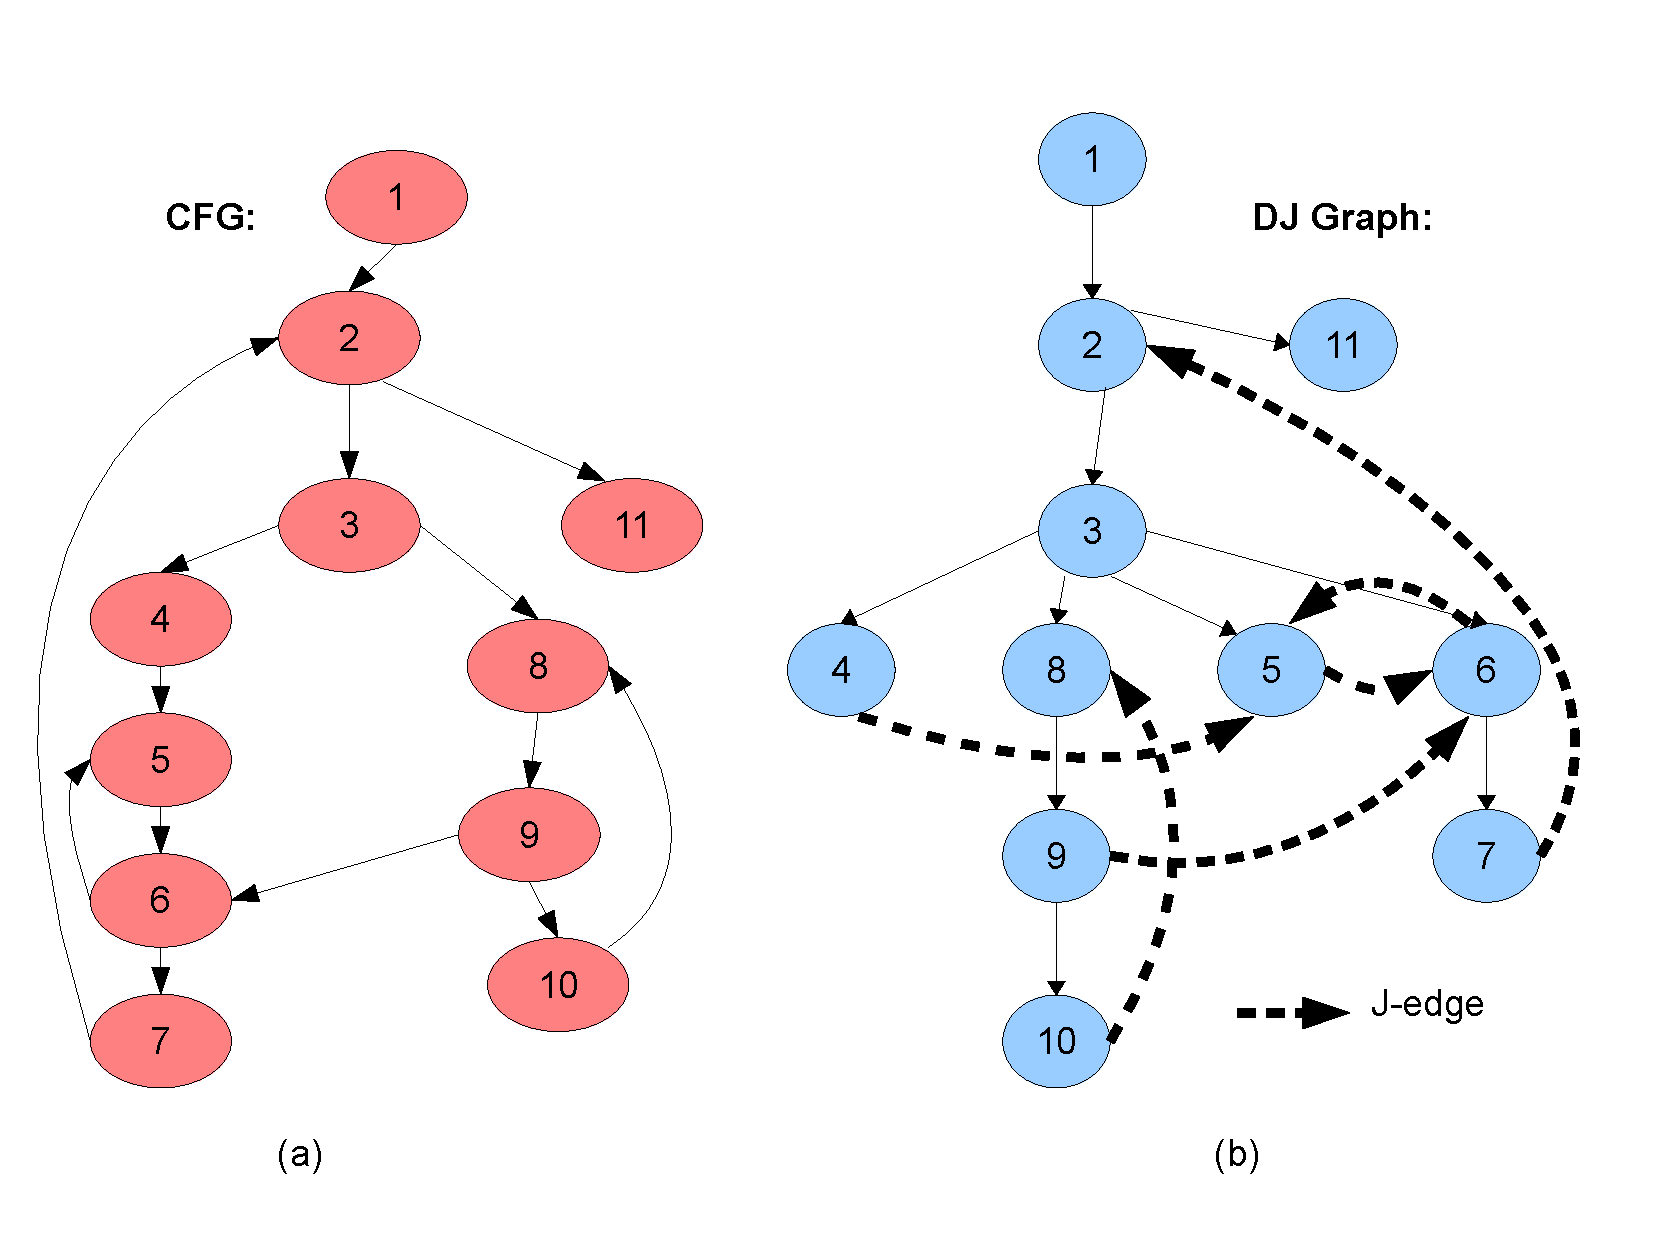
\includegraphics[scale=0.4]{cfglive.pdf}}
    \caption{Motivating Example }
    \label{fig:tdmsc}
    \end{figure} 

Now we can extend the above idea to compute the IDF for a set of nodes, and hence
the set of $phi$-nodes. Given a set of initial nodes $N_{\alpha}$ to compute the 
relevant set of $\phi$-nodes,
Sreedhar and Gao  made two key observations: (1) Let $y$ be an ancestor node of a node $x$ 
on the dominator tree. $If DF(x)$ has
already been computed before the computation of $DF(y)$,  $DF(x)$ need not
be recomputed when computing DF(y). However, the reverse may not be
true, and  therefore the order of the computation of DF is crucial. 
(2) When computing $DF(x)$ we only need to examine J edges $y\st{J} z$, where $y \in SubTree(x)$
and $z$ is a node such that $z.level \leq x.level$

To illustrate the two key observations consider the example DJ graph \ref{fig:tdmsc},
and let us compute $IDF(\{8,9\})$. Now supposing we start with node 8 and compute 
$DF(8)$ using the second key observation. The resulting DF set is $DF(8) = \{6,8\}$. 
Now supposing we next compute the DF set for node 9, and the resulting set is
$DF(9) = \{6,8\}$. Notice here that we visited the edges $9 \st{J} 6$ and
$9 \st{J} 6$ twice, once during the computation of $DF(8)$ and once again
during the computation of $DF(9)$. We can avoid such duplicate visits using the
first key observation by ordering the computation of DF set so that we first compute
$DF(9)$ and then during the computation of $DF(8)$ we avoid visiting the sub-tree of
node 9, and use the result $DF(9)$ that was previously computed. In the next section
we present the Sreedhar and Gao algorithm based on the above key observations.


\subsection{Algorithm}

In this section we present the Sreedhar and Gao algorithm. Let $x.level$ be the
depth of the node from the root node with $root.level= 0$. To ensure that the nodes
are processed according to the first key observation we use  a simple 
$OrderedBucket$ that is nothing more than an array of set. We use two routines
(1) InsertNode($n$) that inserts the node $n$ in the set $OrderedBucket[n.level]$, and
(2) GetNode() that returns a node from the $OrderedBucket$ with largest level number. 
The complete Sreedhar and Gao algorithm is shown in Figure~\ref{F:IDFMain}.

\begin{figure}[!ht]
\centering
\begin{minipage}[t]{3in}
\noindent{\bf Input:} A DJ Graph representation of a program and $N_{\alpha}$.
\noindent{\bf Output:} The set $IDF(N_{\alpha})$.

Procedure IDFMain(Set $N_{\alpha}$) 
\{
\begin{code}
\x1 foreach node $x \in  N_{\alpha}$do
\x2    InsertNode($x$)
\x1 endfor
\x1 while(($z = GetNode() \neq null$)  \label{C:get}
\x2   $croot = z$
 \x2  $x.visited = true$ ;
 \x2  Visit($z$)
\x1 endwile
\end{code}
\} 

Procedure Visit($x$)
\{
\begin{code}
\x1 foreach node $y \in  Succ(x)$
\x2  if($x \st{} y = Jedge$)
\x3   if($y.level < croot.level$)

\x4 if($y \not \in IDF$)
\x5  $IDF = IDF \cup {y}$   \label{C:idf}
\x5    if($y \not  \in N_{\alpha}$)
\x6       InsertNode($y$) \label{C:insert}
\x5  endif
\x4  endif
\x3  endif
\x2 else /* visit D edges */
\x3 if($y.visited = false $)
\x4 $y.visited = true$
\x4 // if($y.boudary == false$)   \label{C:cached}
\x5 Visit($y$) \label{C:dedges}
\x4 // endif
\x3 endif
\x2 endif
\x1 endfor
\end{code}
\} 
\end{minipage}
\caption{Sreedhar and Gao algorithm for computing IDF set.}
\label{F:IDFMain}
\end{figure}

First we insert all nodes in $N_{\alpha}$ in the $OrderedBucket$. The nodes are processed
in a bottom-up fashion over the dominator tree from highest node level to least node level
(step ~\ref{C:get}). The procedure Visit($x$) essentially walks down the  DJ Graph 
and identifies candidate J edges whose destination node are in the $IDF$ set (step \ref{C:idf}).
Notice that at step \ref{C:insert} a node is inserted in the OrderedBucket if it was
never inserted before. Finally at step \ref{C:dedges} we continue to process the nodes
in the sub-tree by visiting over the D edges. When the algorithm terminates the 
set $IDF$ will contain the IDF set for the initial $N_{\alpha}$.

The IDF set can be computed using Pingali and Billardi APT data structure. Recall
that APT data structure is an extension of (cached) DJ graph where the J edges are
cached at ``bounday'' nodes. The only only modification that is needed is to
ensure that we need not visit all the nodes of a sub-tree rooted at a node
$y$. At step\ref{C:cached} if a node $y$ is a boundary node, we avoid visiting 
the subtree rooted at $y$. The reason for this is that at a boundary all the
required J edges are cached. 

Finally, it is straightforward to see that the time complexity of Sreedhar and Gao algorithm is linear.
This is based on the observation that each edge in the DJ Graph is visited on a constant number of
times and the fact that the size of a DJ graph is linear with respect to the size of the
the corresponding control flow graph.


\section{Placing $\phi$-points using Merge Sets}
\subsection{Introduction}

Cytron's algorithm uses the concept of Dominance Frontiers, The collective
size of which can grow as $\Theta(|V|^{2})$, even for structured
programs. Cytron and Ferrante proposed an \emph{on-the-fly }algorithm
which computes $J$-sets in $O(|E|\alpha(|E|))$ time per variable.
However, path compression and other complications made this algorithm
less competitive with CFR in practise.

Sreedhar and Gao's approach that traverses the dominator tree of the
tree of the program to compute $J$-sets on demand. This algorithm
needed $O(|E|)$ preprocessing time, $O(|E|)$ preprocessing space
and query time, and is easy to implement, but is not competitive with
CFR+ for several cases.

Bilardi and Pingali's main contribution are the following: (i) definition
of $Merge$-relations, which provided another way for $\phi$ placement,
independent of $DF$ relation. (ii) a simple
framework in which all the algorithms for $\phi$-placement can be
placed, (iii) two new $O(|V|+|E|)$ algorithms for $\phi$-placement:
pushing and pulling, (iii) an approach to obtain a linear time multiple-variable
$\phi$-placement algorithm in the size of output for general programs.


\subsection{Definitions and Properties}


\paragraph{$Merge$-sets}

$Merge$ is is a binary relation $Merge\subseteq V\times V$ such
that $Merge=\{(w,v)|v\in J(\{START,w\})\}$. For any node $w$, $Merge$-set
of $w$ is $Merge(w)=\{v|(v,w)\in Merge\}$. Intuitively, $Merge(w)$
is the set of nodes where $\phi$-functions must be placed if the
only assignment to the variable are $START$ and $w$. 


\paragraph{Properties of Merge-sets}

It can be proved that $Merge(x)=J^{+}(x)=DF^{+}=IDF(x)$. Further,
$J(S)=N_{\alpha}(S)=\bigcup_{w\in S}Merge(w)$. Hence, $Merge$ relation
and its graph could be used for computing $\phi$-function placement. 

%{[}SOME MORE PROPERTIES?{]}
%
%The given program is irreducible iff its $Merge$ graphs has cycles.
%??? Transitivity of the Merge relation. ????? 


\paragraph{$\alpha-DF$ and $\omega-DF$ }

The $\alpha-DF$ graph: It can be noticed that this graph is the same
as the $J$-edge set of a $DJ$-graph as called by Sreedhar and Gao.
The $\omega-DF$ graph is the graph obtained from $DF$ graph, by
considering only edges which have source and target at the same level
of the dominator tree.

%Diagram of alpha and omega DF graphs based on the original drawing


\subsection{A classification of $\phi$-placement algorithms}

Bilardi and Pingali present a framework in which the various $\phi$-placement
algorithms could be placed.

Firstly, they introduce the concept of Preprocessing time $T_{p}$,
preprocessing space $S_{p}$ and query time $T_{q}$ so that the different
algorithms could be quantitatively compared and classified. They also
introduce a qualitative framework in which the algorithms could be
classified. The classes in this framework are Two-phase, Lock step
and Lazy algorithms, with the type of scans being edge-scan, node-scan and
the direction of traversal of being either top-down or bottom-up.

The algorithms of CFR+, Sreedhar and Gao, Pingali and Bilardi 1995,
among others are classified into this framework.


\paragraph{Two-phase Algorithms}

Two-phase algorithms compute the entire $DF$ graph in a preprocessing
phase before doing reachability computation to answer queries of $\phi$-placement.
They are either \emph{edge-scan }or \emph{node-scan }algorithms. The
node-scan algorithm proposed by Bilardi and Pingali is similar to
the CFR+. The edge-scan algorithm that Bilardi and Pingali proposed
is new. Two-phase algorithms suffer from the
same drawback as CFR because of the asymptocally quadratic size of
DF sets.


\paragraph{Lock-step algorithms}

Lock step algorithms interleaves the computation of $DF^{+}(S)$ with
that of the $DF$ relation. They are either of the \emph{pulling }or
\emph{pushing }variety. A pulling (respectively pushing) algorithm
adds the current node to $DF^{+}(S)$ if any of its predecessors (respectively
successors) in the $DF$ graph belongs to $S$ if it has not been
previously added. Also, the pulling (respectively pushing) algorithm is
a variation of the edge-scan (respectively node-scan) algorithm proposed
in the category of two-phase algorithms. $\omega$-ordering 

%Need to add the algorithm(s).


\paragraph{Lazy algorithms}

Lazy $\phi$-placement algorithms compute $DF^{+}$ only on a demand-driven
basis. A factor $\beta$ could be defined so that algorithms could
be classified on how much percentage of $EDF$ are cached.


\subsection{New linear-time $\phi$-placement algorithms}


\paragraph{Node Scan}

Similar to CFR+. 

As DF graph is comparable in size to CFG, two-phase algorithms may
be quite efficient.


%\subsection{An approach for linear-time multi-variable $\phi$-placement algorithms}
%{[}With space constraint, this sub-section can be removed{]}
%What really makes the case for M relation wrt. the J relation?


%    This section will discuss Pingali and Bilardi's algorithms on computing $\phi$- points
%    using Merge Sets. Total Length {\bf[2-3 pages]}, Key Author {\bf[Sreedhar, Dibyendu - backup]}.
%
%\subsection {Basics}
%    Introduce Merge, as well as $\alpha$-DF and $\omega$-DF graphs. Augmented Dominator Tree(?). Discuss 
%    how Sreedhar's and Bilardi-Pingali algos have common ground.
%
%\subsection{Algorithms}
%    Pseudo-codes of 2-phase, Lock-Step and Lazy Algorithms ( all reqd ?). Mention the complexities
%    along with the algos.
%


\section{Fast and Practical $\phi$-placement using Merge Sets and DJ Graphs}

As it has been previously indicated, since the time of CFR, all algorithms,
except the lazy computation use the $DF$-sets in some form or other.
But, $DF$-sets not really needed, other than for $\phi$ placement.
And, $DF$-set computation could be costly, taking quadratic time
for some examples as shown in CFR.

As shown in the previous section, $DJ$-graph construction is very
cheap. It can be done by annotating the along Dominator tree with
$J$-edges or by copying the CFG with labelling all edges as J-edges,
then rename the edges that are in $D$-Tree as $D$-edges. In either
of the methods, it is available in linear-time in CFG size, with very
low constant. Space complexity of $Merge$ sets is comparable to that of $DF$-sets.


\subection{Iterative Merge Set Computation}

The following definitions are needed for explaining Das and Ramakrishna's
algorithms.


\paragraph{Shadow}

Given a $e:s\rightarrow t$, $Shadow(e)$ is the set of nodes on the
simple path in the dominator tree from node $s$ to node $idom(t)$,
excluding node $idom(t)$ itself i.e., $\forall x\in Shadow(e)$,
$x\, dominates\, s$ but does not strictly dominate $t$. 


\paragraph{Inconsistency Condition }

If the $source(s)$ and $target(t)$ of a $J$-edge do not satisfy
$Merge(s)\supseteq Merge(t)$, then the nodes in the shadow of the
$J$-edge are said to be inconsistent.

\subsection{TDMSC-I}

%==
%
%\textbf{Algorithm: Top Down Merge Set Computation (TDMSC-I)}
%
%Input: $DJ$-graph
%
%Outputs: a. Partial/Complete Merge Sets for every node of the $DJ$-graph
%
%b. A boolean value to indicate whether a subsequent pass is required
%
%RequireAnotherPass=False;
%
%\textbf{while}(in B(readth) F(irst) S(earch) order) do
%
%Let $n$ $=$ Next Node in BFS list
%
%\textbf{for} (all incoming edges to $n$) do
%
%Let $e$ $=$ Incoming edge
%
%\textbf{if} ($e$ is a $J$-edge $\wedge$ $e$ not visited) then
%
%$Visit(e)$ 
%
%Let $snode$ $=$ Source Node of $e$
%
%Let $tnode$ $=$ Target Node of $e$ 
%
%Let $tmp$ $=$ $snode$
%
%Let $lnode$ $=$ $NULL$
%
%\textbf{while} $(level(tmp)\ge level(tnode))$ do
%
%$Merge(tmp)=Merge(tmp)\bigcup Merge(tnode)\bigcup\{tnode\}$
%
%$lnode=tmp$
%
%$tmp=parent(tmp)$ //dominator tree parent
%
%end while
%
%\textbf{for} (all incoming nodes to $lnode$) do //$lnode$ ancestor
%of $snode$
%
%Let $e'$ $=$ Incoming edge
%
%\textbf{if} ($e'$ is a $J$-edge $\wedge$ $e'$ visited) then
%
%Let $snode'$ $=$ Source Node of $e'$
%
%\textbf{if} $(Merge(snode')\nsupseteq Merge(lnode))$ then //Check
%inconsistency
%
%RequireAnotherPass = True
%
%\textbf{end if}
%
%\textbf{end if}
%
%\textbf{end for}
%
%\textbf{end if}
%
%\textbf{end for}
%
%\textbf{end while}
%
%return RequireAnotherPass
%
%==
    \begin{figure}[htb]
    \centerline{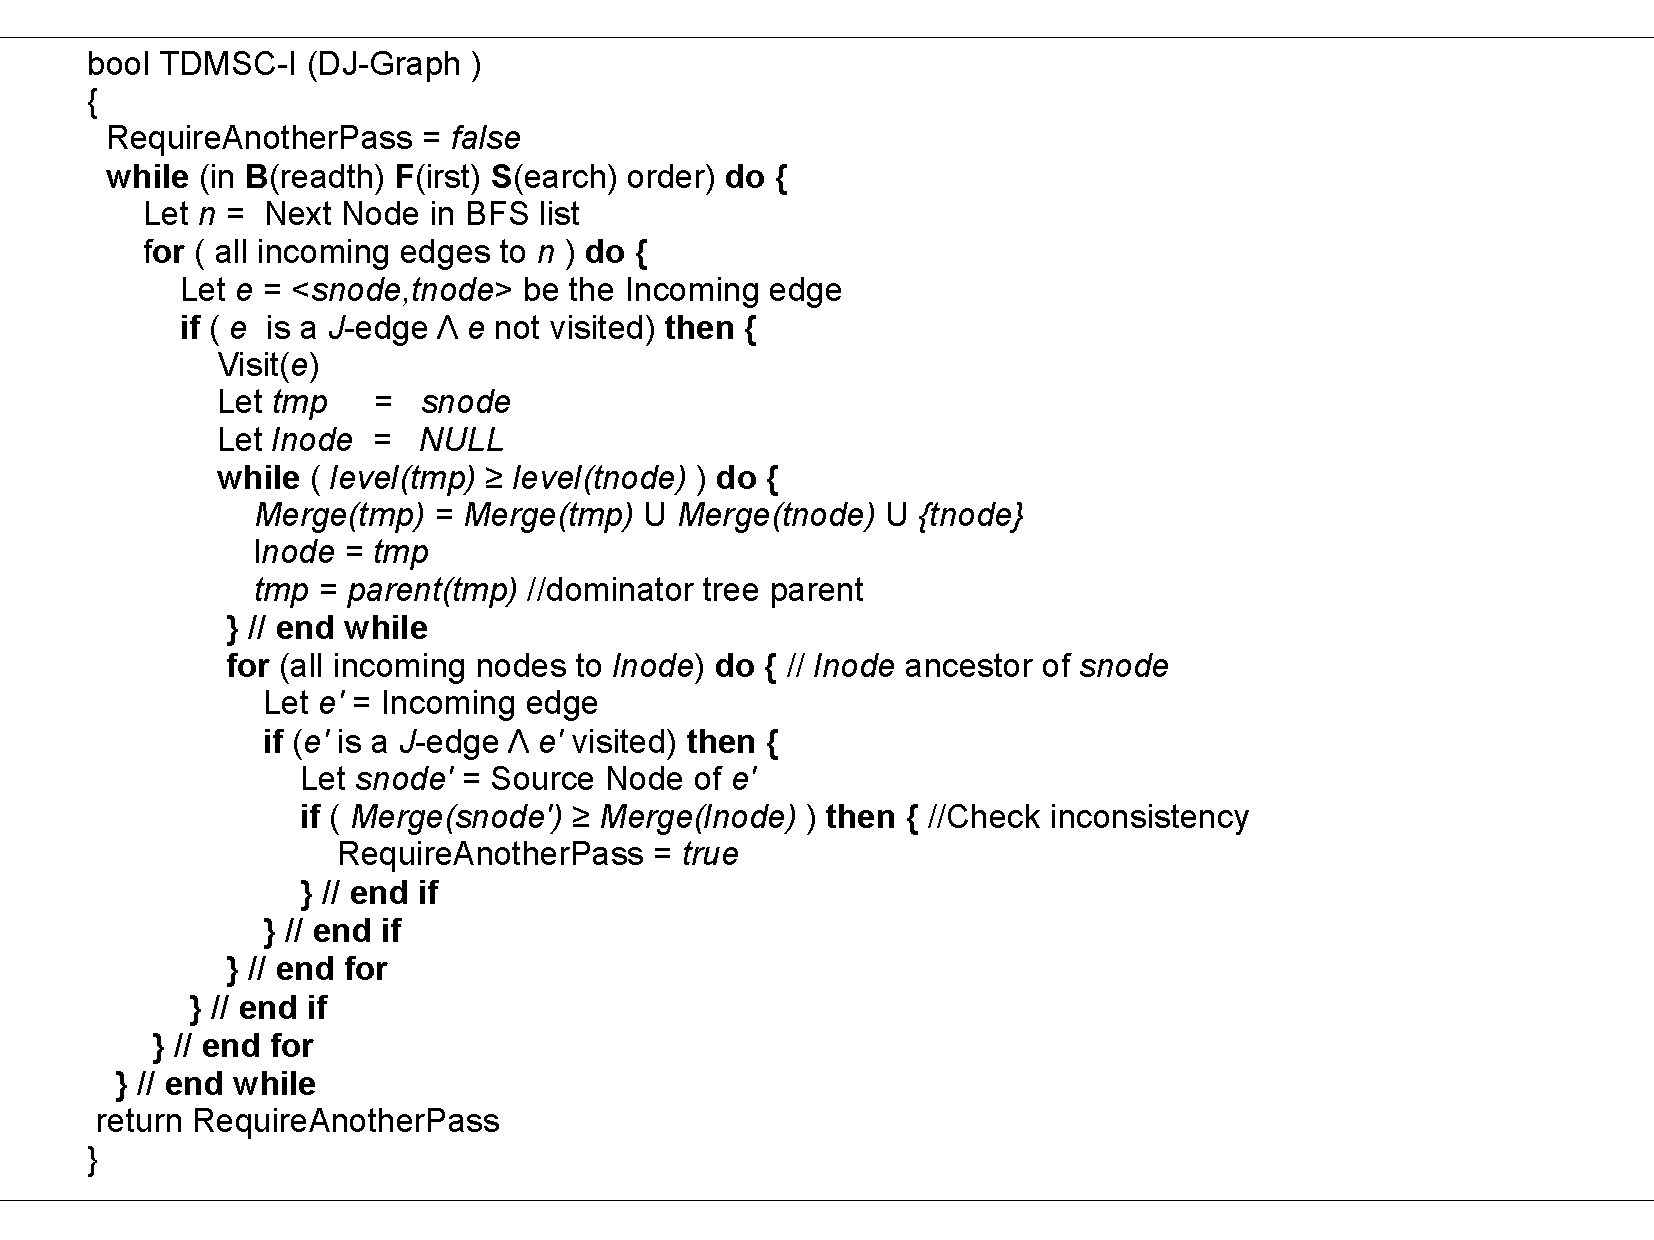
\includegraphics[scale=0.4]{tdmsc-i.pdf}}
    \caption{TDMSC-I Algorithm }
    \label{fig:tdmsc}
    \end{figure} 


The algorithm of TDMSC-I is enclosed in another algorithm that repeatedly
calls it till RequireAnotherPass is false.


\subsubsection{TDMSC-II}

Das and Ramakrishna term as TDMSC-II, an improvement to algorithm
TDMSC-I. This improvement is fueled by the observation that for an
inconsistent $J$-edge, the merge sets of all nodes in the shadow
of that edge can be locally corrected for some special cases. This
heuristic works very well for certain class of problems -- especially
for CFGs with DF graphs having $2$-chains and simple-cycles. This
eliminates an extra pass as an inconsistent node is made consistent
immediately on being detected. 

Das and Ramakrishna's TDMSC-II has this additional step immediately
after the inner while loop of TDMSC-I.


\subsection{Complexity}

A single pass of TDMSC-I can be shown to have a complexity of $O(|V|+|E|)+O(h^{avg}*|J|)+O(e^{avg}*|J|)$.
For total running time, this has to be multiplied by an additional
factor of $P$, where $P$ is the number of passes that are needed
to reach fixed points for merge sets. On average, this overall complexity
drops down to linear time, if the following factors are taken into
account: CFGs usually are sparse, both $h^{avg}*|J|$ and $e^{avg}*|J|$
are of the order of $O(|V|)$, and $P$ is a small constant.


%\subsection{Empirical results}

%Both the above algorithms have been implemented in the High Level
%Optimizer of HP's PA C Compiler, and later in the ST-compiler. From
%the first implementation, the following are the results: 

%The size of $Merge$-sets is almost similar to $DF$-sets, and small
%enough to be stored in small bitsets. As noted earlier, $DJ$ graph
%comes almost for free after the Dominance-tree computation.

%Among the nearly $57K$ cases from SpecInt2000, $75\%$ of all cases
%stabilizes in a single top down pass of algorithm TDMSC-I, while nearly
%$25\%$ of cases stabilize in two passes. Only in around $0.5\%$
%cases is a third pass of the algorithm required. These numbers further
%drop down with the improvement suggested in TDMSC-II. In this, the
%number of cases where a second pass is required is reduced to $5\%$,
%and the number of cases when a third pass is required is just $3$. 

%Also, TDMSC-II gives around $17\%$ of improvement in compile time
%for SpecInt2000 and around $37\%$ improvement for the SpecFP2000
%benchmarks, when compared with CFR+. (This time is \emph{inclusive
%}of time to compute Merge-sets as well as time to compute $\phi$-points
%for all $N_{\alpha}$.)

\section{Computing Iterated Dominance Frontier Using Loop Nesting Forests}
    This section illustrates the use of {\bf loop nesting forests} for construction of the iterated
    dominance frontier (IDF) of a set of vertices in a CFG, which may contain both reducible as well as
    irreducible loops.

    \subsection{Loop nesting forest}
     Loop nesting forest is a data structure that respresents the loops in a CFG
    and the containment relation between them. However, while there is a fairly accepted notion of
    loop nesting forest in a reducible graph \cite{morgan_book}, there is less agreement about their
    definition in arbitrary graphs. Steensgard \cite{steensgard}, Sreedhar \cite{sreedhar} and Havlak
    \cite{havlak} all provide different definitions which have merits under different situations. 
    For the example shown in Figure ~\ref{fig:lnf} the loops with backedges $11 \rightarrow 9$ and
    $12 \rightarrow 2$ are both reducible loops.

    \begin{figure}[htb]
    \centerline{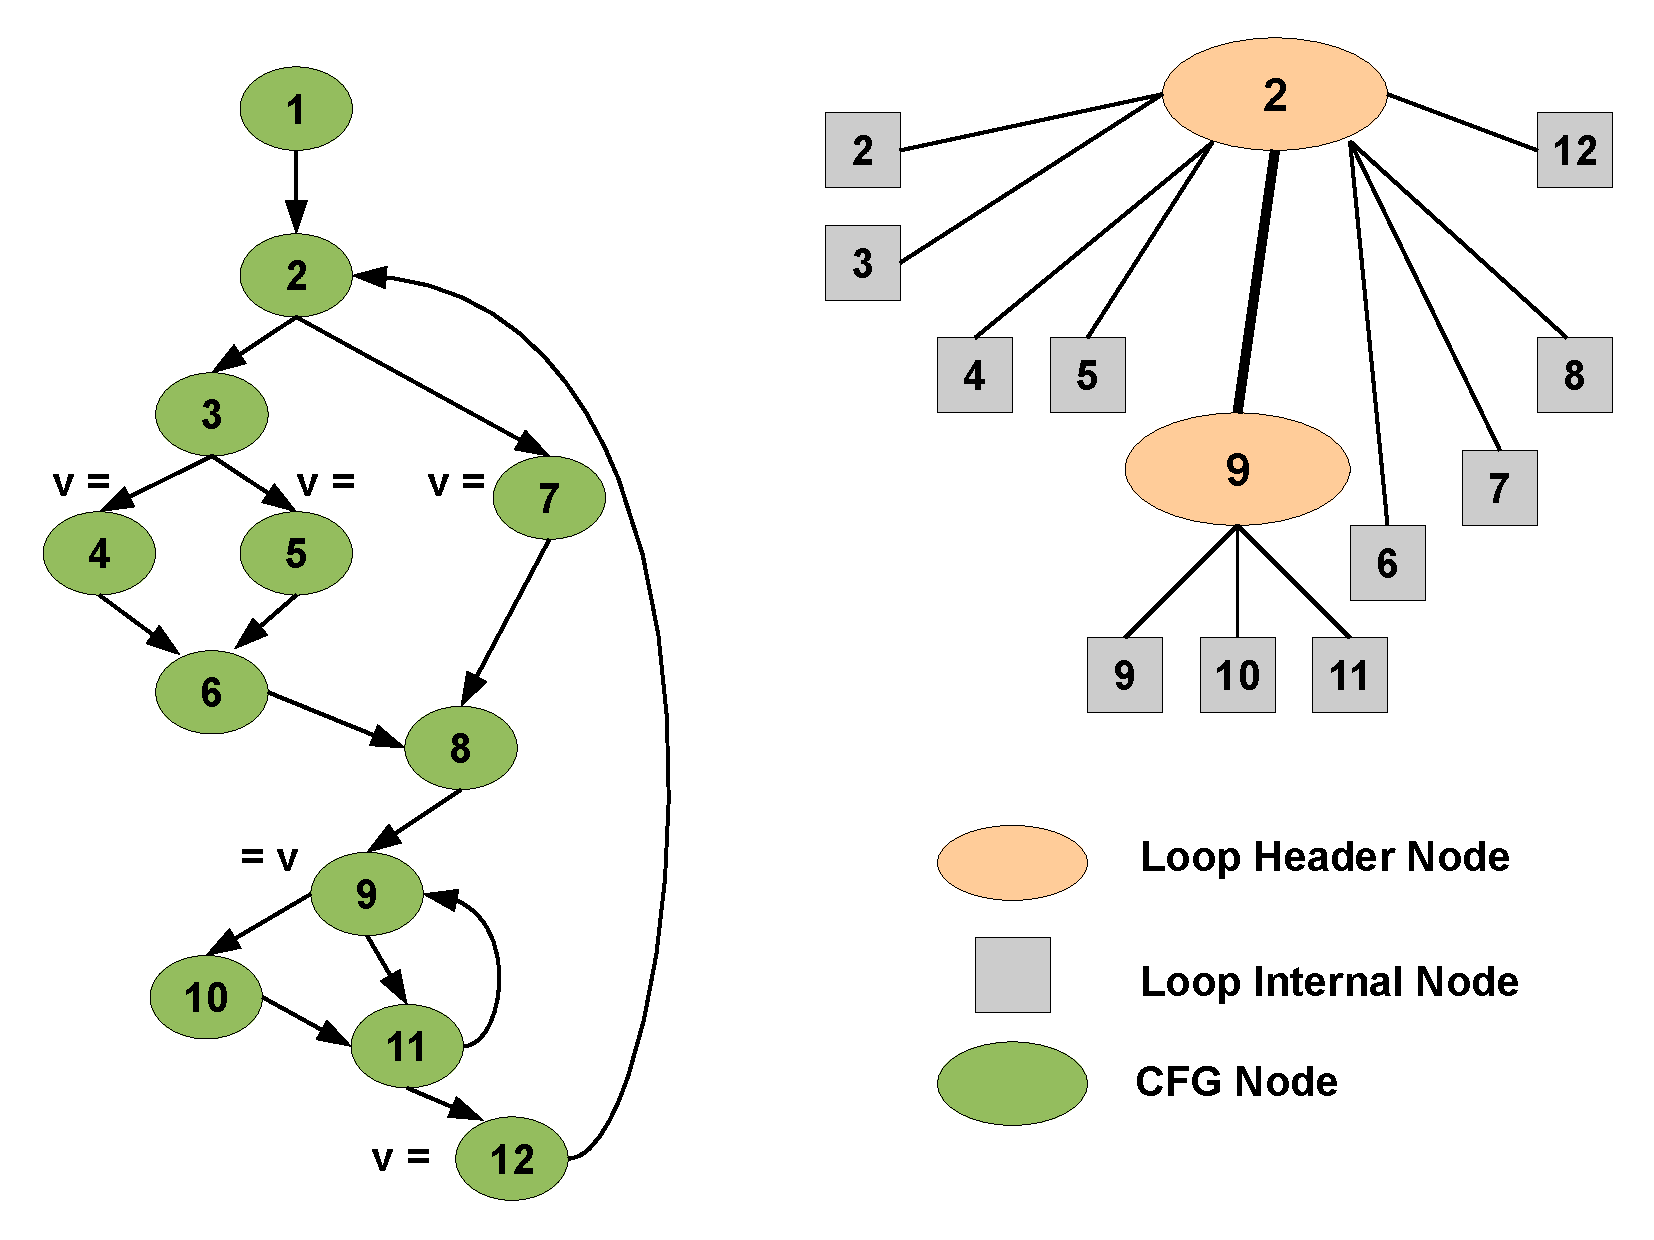
\includegraphics[scale=0.25]{lnfred.pdf}}
    \caption{An example CFG and IDF Computation Using Loop Nesting Forest }
    \label{fig:lnf}
    \end{figure} 

    The corresponding loop nesting forest shown in Figure ~\ref{fig:lnf}(b), consists of two loops
    with their headers given by $2$ and $9$. The loop with header node $2$ contains the loop with 
    header node $9$.
    The algorithm in Figure ~\ref{fig:idfcode} depicts how the IDF can be computed for a set of nodes for an acyclic
    graph $G_{ac}$. The acyclic graph $G_{ac}$ of a graph $G$ with reducible loops can be derived by
    dropping the backedges of the loops. For Figure ~\ref{fig:lnf}, the $G_{ac}$ is formed by dropping
    the backedges $11 \rightarrow 9$ and $12 \rightarrow 2$.
    %\noindent
    \begin{figure}[htb]
    \centerline{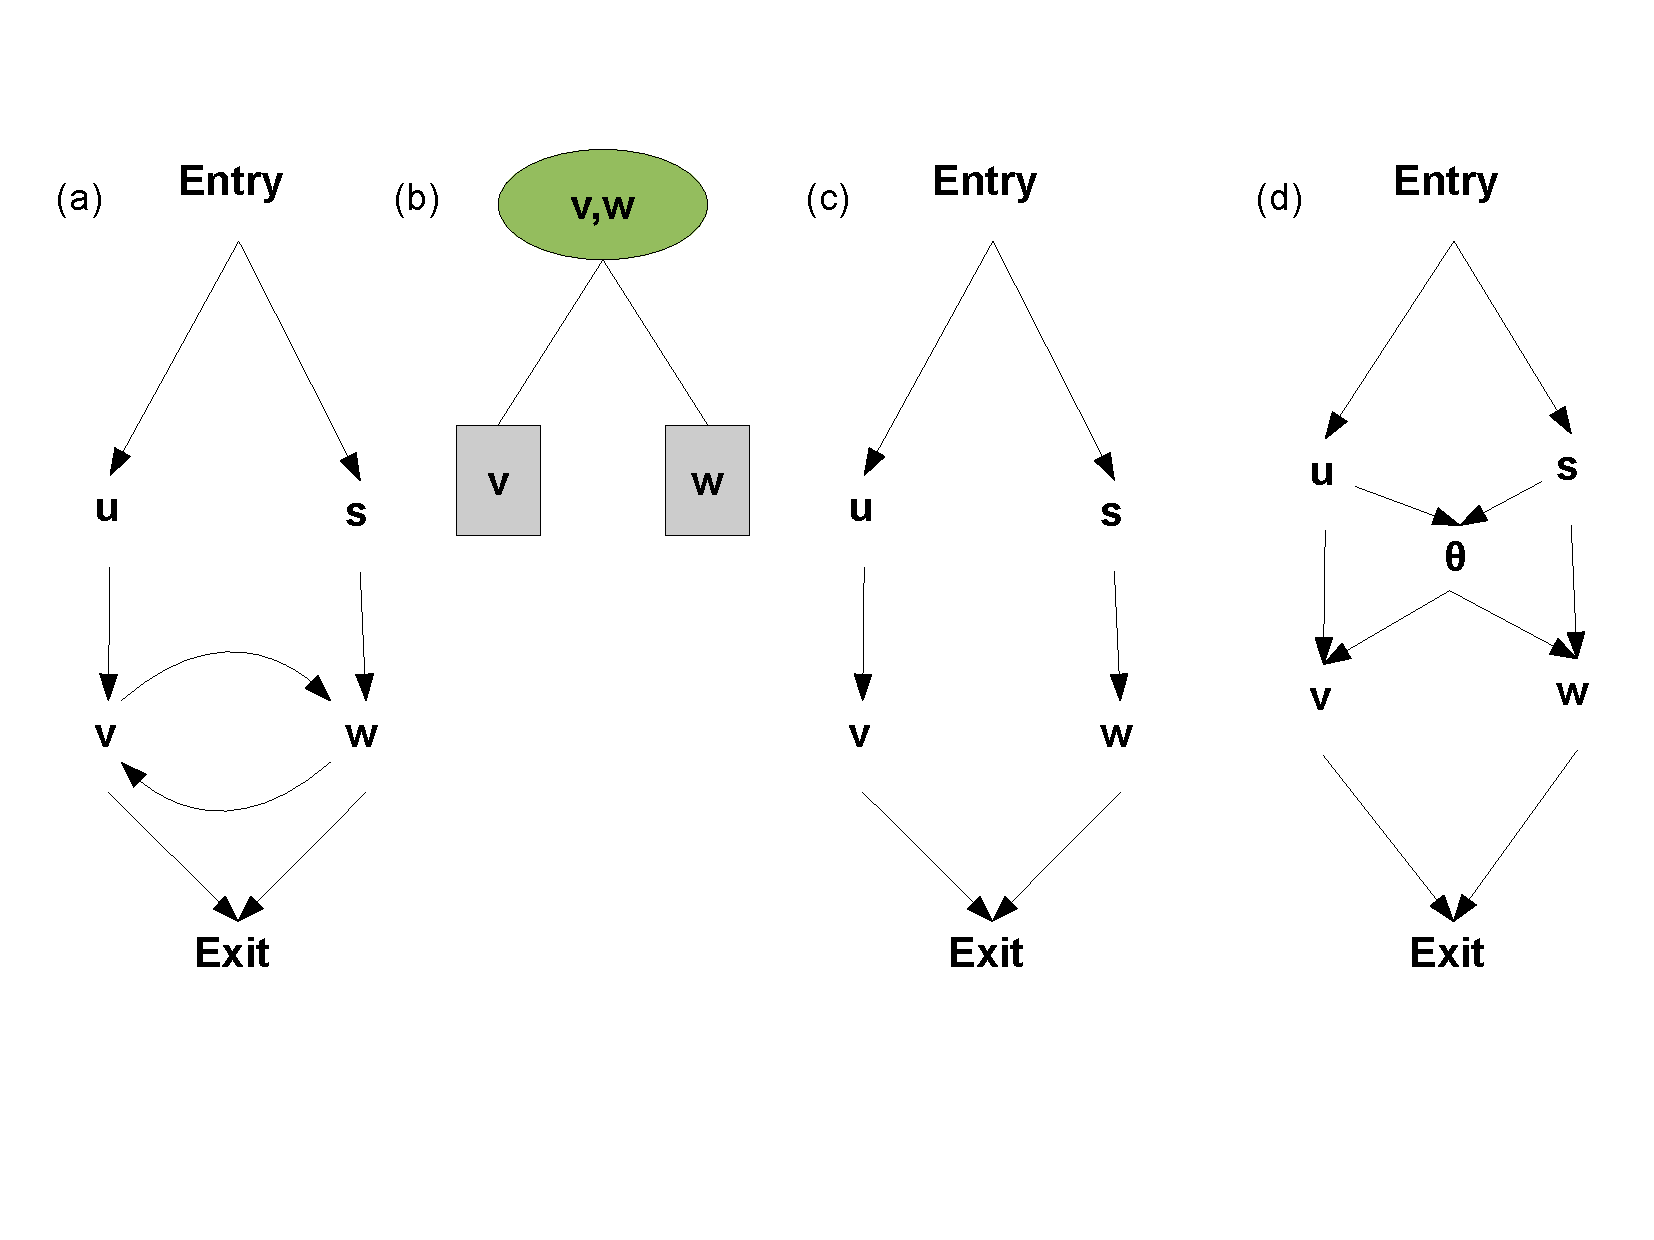
\includegraphics[scale=0.3]{irred.pdf}}
    \caption{(a) An irreducible graph (b) The Loop Nesting Forest (c) The acyclic subgraph (c) Transformed
    Graph}
    \label{fig:irred}
    \end{figure}  


    \begin{figure}[htb]
    \centerline{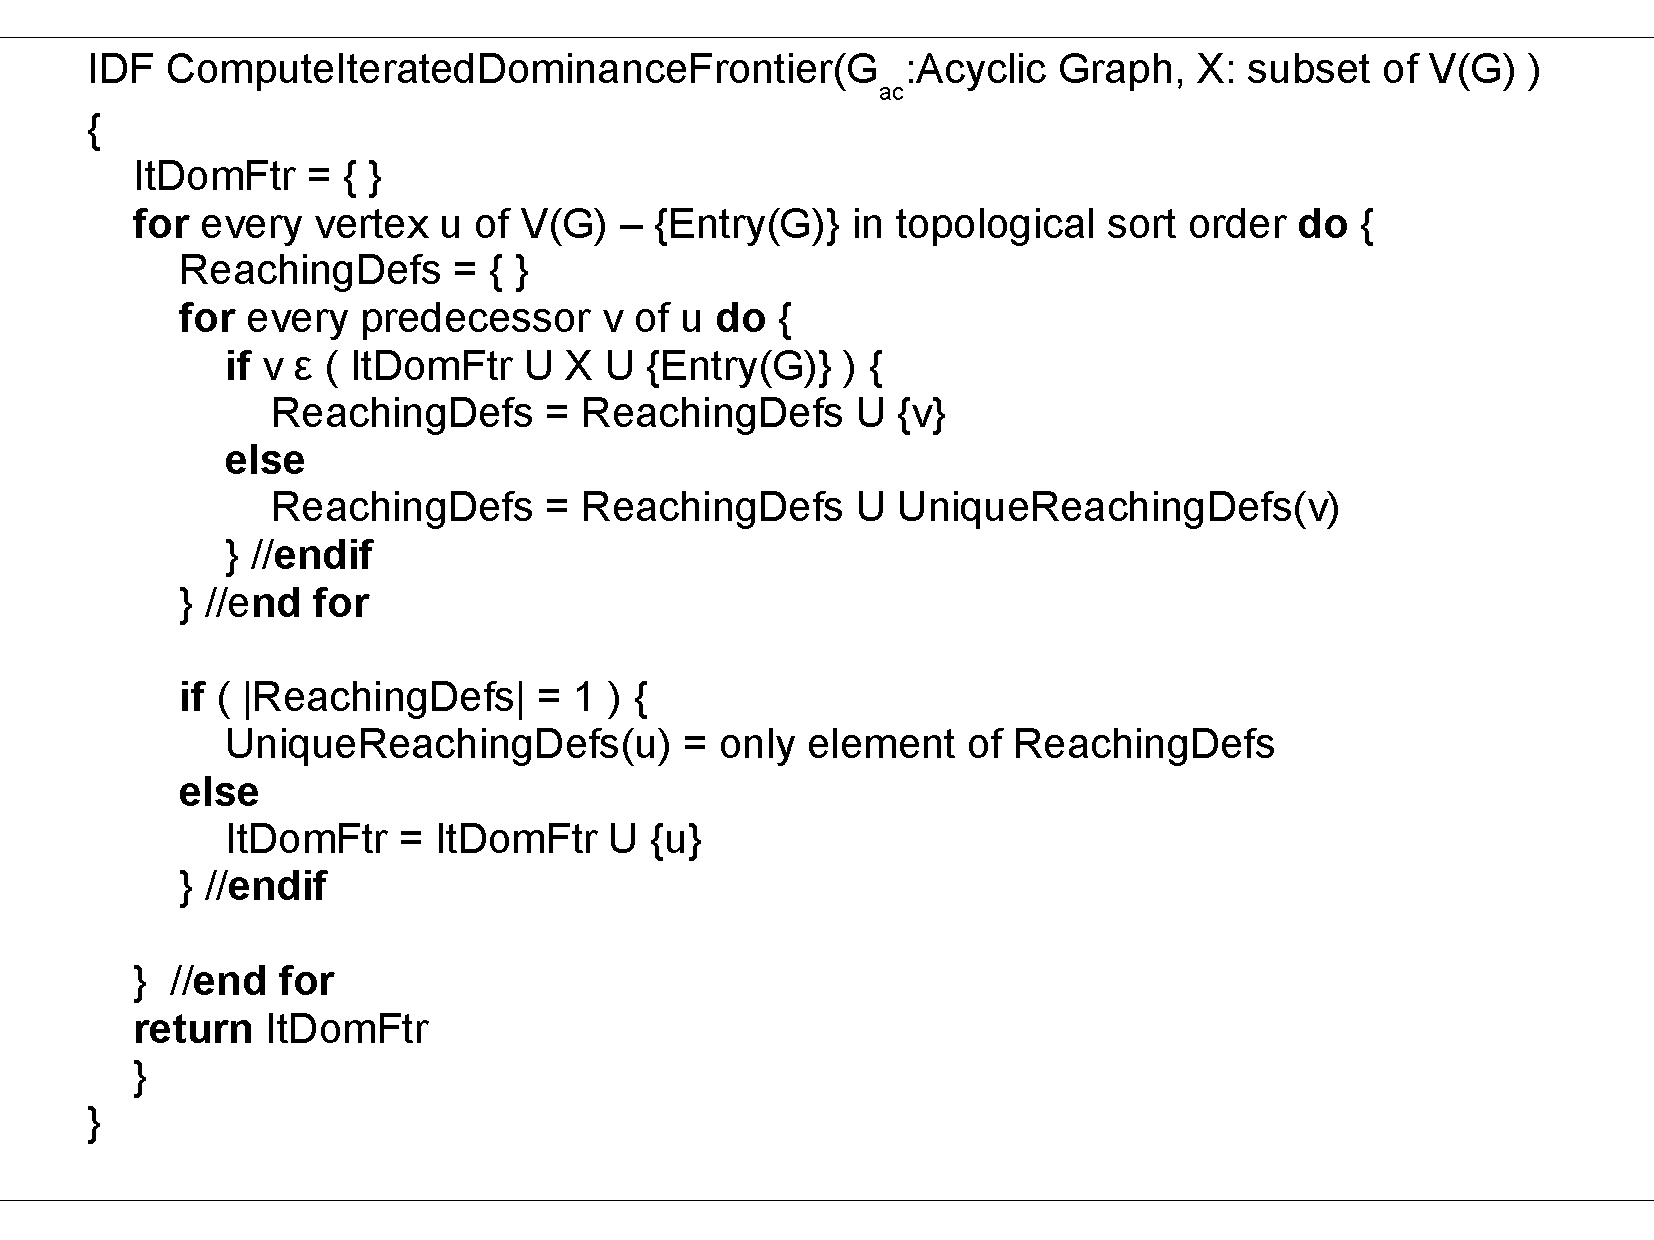
\includegraphics[scale=0.3]{idfcode.pdf}}
    \caption{Pseudocode for computing IDF of an acyclic graph }
    \label{fig:idfcode}
    \end{figure}  
    
    %\hline
    %\noindent
    %ComputeIteratedDominanceFrontier($G_{ac}$:Acyclic Graph,X: subset of $V(G)$)\\
    %\{\\
    %\hspace*{1cm} ItDomFtr = \{ \} \\
    %\hspace*{1cm} {\bf for} $\forall u$ of $V(G) � \{Entry(G)\}$ in topological sort order {\bf do} \{ \\
    %\hspace*{2cm}   ReachingDefs = \{ \} \\
    %\hspace*{2cm}   {\bf for} $\forall$ predecessor $v$ of $u$ {\bf do} \{ \\
    %\hspace*{3cm}      {\bf if} $v in$ ( ItDomFtr $\cup$ X $\cup \{Entry(G)\}$ ) \{ \\
    %\hspace*{4cm}         ReachingDefs = ReachingDefs $\cup \{v\}$ \\
    %\hspace*{3cm}     {\bf else} \\
    %\hspace*{4cm}        ReachingDefs = ReachingDefs $\cup$ UniqueReachingDefs($v$) \\
    %\hspace*{3cm}   \} //endif \\
    %\hspace*{2cm}  \} //end for \\
    %\hspace*{2cm}   {\bf if} ( $\|$ReachingDefs$\|$ = 1 ) \{ \\
    %\hspace*{3cm}      UniqueReachingDefs($u$) = only element of ReachingDefs \\
    %\hspace*{2cm}   {\bf else} \\
    %\hspace*{3cm}     ItDomFtr = ItDomFtr $\cup \{u\}$ \\
    %\hspace*{2cm}  \} //endif    
    %\hspace*{1cm}  \}  //end for \\
    %\hspace*{1cm}{\bf return} ItDomFtr \\   
    %\} \\
    %\hline



    How can the above algorithm be extended to handle reducible graphs? A reducible graph can be
    decomposed into an acyclic graph and a set of backedges. The contribution of backedges to the
    iterated dominance frontier can be identified by using the loop nesting forest. If a vertex $u$
    is contained in a loop then $IDF(u)$ will contain the loop header. For any vertex $u$, let $HLC(u)$
    denote the set of loop headers of the loops containing $u$. Given a set of vertices $X$, it turns
    out that $IDF(X) = HLC(X) \cup IDF_{ac}(X \cup HLC(X))$ where $IDF(X)$ and $IDF_{ac}$
    denote the IDF over the original graph $G$ and the acyclic graph $G_{ac}$ respectively. Reverting
    back to Figure ~\ref{fig:lnf} we see that in order to find the $IDF$ for the nodes where the variable 
    $v$ is defined, we need to evaluate $IDF(\{4,5,7,12\})$. Firstly, we would need to evaluate 
    $IDF_{ac}(\{4,5,7,12\} \cup HLC(\{4,5,7,12\}))$. $HLC(\{4,5,7,12\}) = \{2\}$ as all these nodes are contained 
    in a single loop with header $2$. Hence, we would need to find $IDF_{ac}(\{2,4,5,7,12\})$ which turns
    out to be the set $\{6,8\}$. Finally, $IDF(\{4,5,7,12\}) = HLC(\{4,5,7,12\}) \cup \{6,8\} = \{2,6,8\}$.

    %\begin{figure}[htb]
    %\centerline{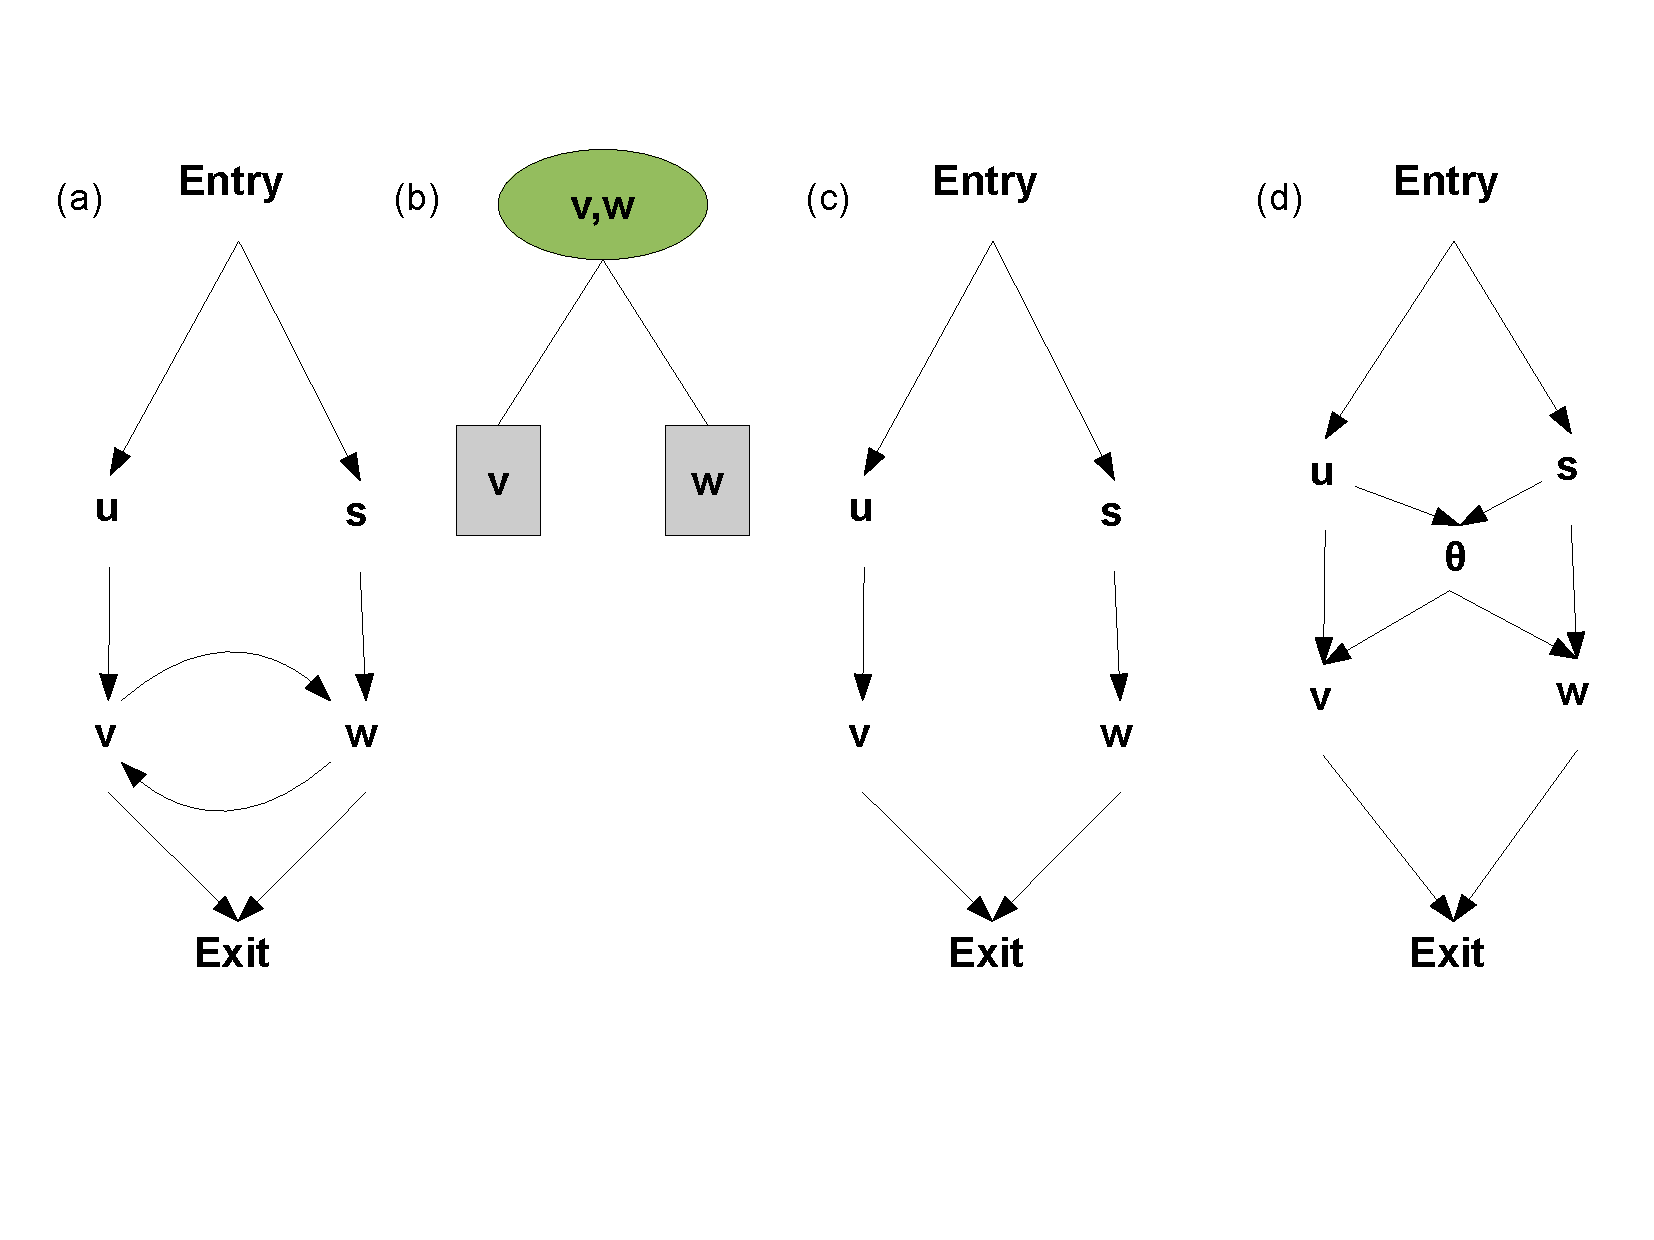
\includegraphics[scale=0.3]{irred.pdf}}
    %\caption{(a) An irreducible graph (b) The Loop Nesting Forest (c) The acyclic subgraph (c) Transformed
    %Graph}
    %\label{fig:irred}
    %\end{figure}  

    Now that we have shown how IDF can be computed for graphs with reducible loops using 
    loop nesting forests, we will briefly touch
    upon how graphs containing irreducible loops can be handled. The trick behind the implementation
    is to transform the irreducible loop in such a way that an acyclic graph is created from the loop
    without changing the dominance properties of the nodes. Referring to Figure ~\ref{fig:irred}, we see 
    that the irreducible loop comprising of nodes $v$ and $w$ in (a) can be transformed to the acyclic
    graph in (c). We can now create a new dummy node $\theta$ and add edges from the predecessor of all
    the header nodes of the acyclic graph to $\theta$, as well as add edges from $\theta$ to all the 
    header nodes. The crucial observation that allows this transformation to create an equivalent acyclic
    graph is the fact that the dominator tree of the transformed graph remains identical to the
    original graph containing an irreducible cycle. One of the drawbacks of the transformation is the
    possible explosion in the number of dummy nodes and edges for graphs with many irreducible cycles. This
    can be kept under control by utilizing a single dummy node which acts as the sink for all the edges
    emanating from the predecessors of the headers while acting as a source for all the edges terminating
    at the headers.

    \section{Concluding remarks}


    \noindent
    {\bf Note:} It is assumed ( for all the sections ) that we do not need to provide lemmas/proofs. 
    We can probably state the major observations as part of the first subsection of each section 
    ( my reading of the discussions ). A first cut of the page count is around around 14 pages. 12 pages 
    maybe difficult.We can see about that later.

    %\appendix
    %\include{history}       % include first appendix
    %\include{tables}        % include second appendix, etc.
  
    %\backmatter

    %\include{bibliography}  % include bibliography
    %\printindex
         % include index

\end{document}                 
